% !TEX root = ../main.tex

\clearpage
% Source PDF page 4.
\section{第一章\quad 绪论}

为什么当下的大学生如此喜欢奶龙和奶蛙？一只黄皮绿眼睛捧腹大笑的生物，凭什么在校园攻城略地、获粉无数？这是我们不得不思考的问题。~(见\figref{fig:01-1})

% !TEX root = ../../main.tex
\begin{figure}[H]
  \centering
  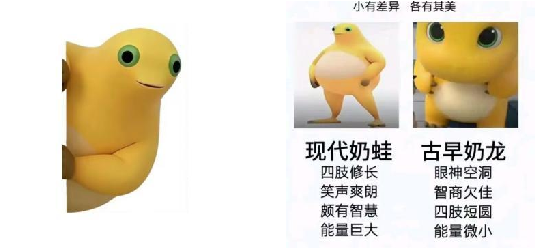
\includegraphics[width=218.62bp,height=0.76\textheight,keepaspectratio]{figures/chapter01/figure01_1.pdf}
  \renewcommand{\thefigure}{1.1}
  \caption{探头偷看的奶蛙（左）和“有点小差异，各有各的美”（右）}
  \label{fig:01-1}
\end{figure}


当下，奶龙同好会在相当一部分高校（例如上海交通大学）的热度和受欢迎程度，已经远远超越了一些小型社团。为什么越聪明的人反而越喜欢那些无厘头、不着边际的东西？本书将从捧腹大笑思想理论体系和奶龙史两个方面深入探讨奶龙的魅力之谜。

我们平时所说的奶龙一般指两种。一种是官方动画的奶龙。~(见\figref{fig:01-2})

% !TEX root = ../../main.tex
\begin{figure}[H]
  \centering
  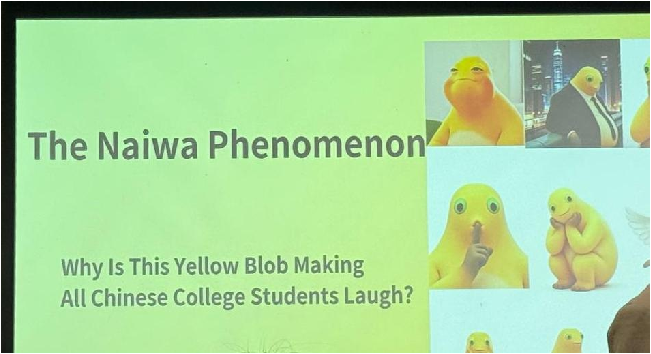
\includegraphics[width=79.7bp,height=0.76\textheight,keepaspectratio]{figures/chapter01/figure01_2.pdf}
  \renewcommand{\thefigure}{1.2}
  \caption{奶龙的官方形象}
  \label{fig:01-2}
\end{figure}


一种则是受到更多追捧的奶蛙。~(见\figref{fig:01-3})

% !TEX root = ../../main.tex
\begin{figure}[H]
  \centering
  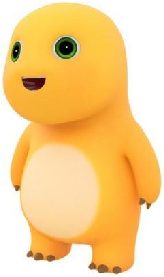
\includegraphics[width=206.38bp,height=0.76\textheight,keepaspectratio]{figures/chapter01/figure01_3.pdf}
  \renewcommand{\thefigure}{1.3}
  \caption{奶蛙经典形象}
  \label{fig:01-3}
\end{figure}


我们在本书中进行区分，不过平时的大多数时间，奶蛙都会被简称为奶龙。因此，大多数情况下奶龙同好会本质是奶蛙同好会，不这样的话会埋下祸根。

